\chapter{Materiał i metoda badawcza}

%W ramach pracy przeprowadzone zostały badania dotyczące klasyfikacji choroby Parkinsona.
%Głównym celem było opracowanie efektywnego modelu klasyfikacji binarnej, który może rozróżniać
%osoby chore na chorobę Parkinsona od osób zdrowych na podstawie analizy sygnałów mowy.
%Przyjęte podejście opiera się na wykorzystaniu metod przetwarzania sygnałów mowy oraz
%uczenia maszynowego. Najpierw zebrano dane, w tym nagrania głosowe osób z chorobą Parkinsona
%(PD) oraz osób zdrowych (HC, ang. \emph{Healthy Controls}). Następnie przeprowadzono analizę przy użyciu różnych ustawień
%spektrogramów i melspektrogramów. Obejmuje to zmienne parametry takie jak rozmiar okna i
%przesunięcie okna. Dodatkowo, przeprowadzono badania dotyczące różnych architektur
%konwolucyjnych sieci neuronowych. Celem jest zbadanie, które architektury sieci i ustawienia
%spektrogramów dają najlepsze wyniki w klasyfikacji choroby Parkinsona dla poszczególnych
%samogłosek. Przeprowadzona analiza porównawcza pozwala na lepsze zrozumienie wpływu tych
%czynników na skuteczność klasyfikacji. W rezultacie, możliwe będzie ustalenie optymalnych ustawień i
%architektur dla klasyfikacji choroby Parkinsona na podstawie analizy sygnałów mowy. Ponadto zbadano
%wpływ rozszerzenia zbioru danych o dodatkowe nagrania pochodzące od tych samych osób.
%
%\begin{figure}[htbp]
%	\centering
%	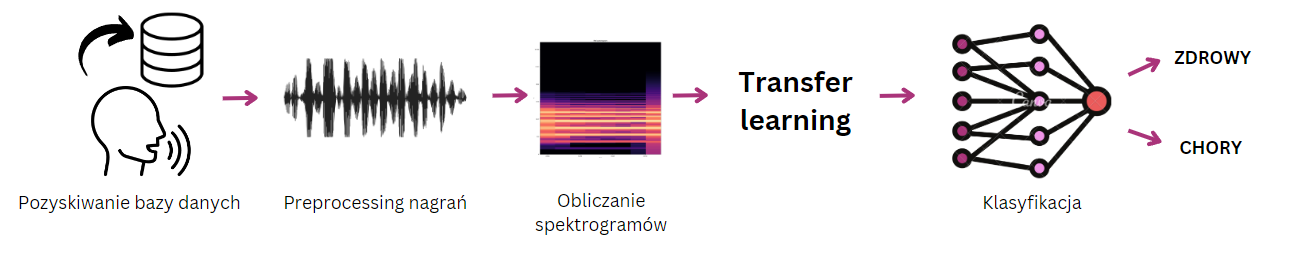
\includegraphics[width=1\textwidth]{./img/methodology}
%	\caption{Schemat przyjętej metody badawczej [opracowanie własne]}
%    \label{fig:methodology}
%\end{figure}

%---------------------------------------------------------------------------

\section{Materiał badawczy}
\label{sec:material-badawczy}
%
%Materiałem badawczym w niniejszej pracy magisterskiej są nagrania głosowe samogłosek: /a/,
%/e/, /i/, /o/ oraz /u/.
%Baza danych obejmuje nagrania osób zdrowych oraz z chorobą  Parkinsona.
%
%[Opis źródła nagrań osób chorych]
%Autorka pracy wykonała nagrania głosu u osób z chorob ˛a Parkinson’a w Krakowskim Szpitalu Specjalistycznym im. Jana Pawła II. Nagrania obejmowały wypowiedzenie samogłosek /a/,
%/e/, /i/, /o/ oraz /u/ w przedłuzonej intonacji przez 27 pacjentów. Pierwszy pomiar wyst˛epował ˙
%wtedy, kiedy u pacjenta zdiagnozowano zupełne wysycenie leków łagodz ˛acych objawy choroby. Nast˛epnie lekarz podawał lek lewodopy. Kolejne pomiary wykonano po 30, 60, 120 i 180
%minutach od spozycia leku. Przed ka ˙ zdym pomiarem, lekarz neurolog wykonywał badanie i ˙
%opisywał stan pacjenta w skali UPDRS.
%
%Nagrania osób zdrowych zostały zebrane w ramach pracy przy wykorzystaniu aplikacji Easy
%Voice Recorder, która jest programem do nagrywania dźwięku. Przed przystąpieniem do pozyskiwania
%danych zapoznano się z charakterystyką problemu. Na podstawie literatury wyróżniono płeć, wiek oraz
%język ojczysty jako czynniki, które mogą wpływać na wyniki klasyfikacji. Zbiór danych powinien być
%zrównoważony pod kątem tych aspektów, tak by nie dopuścić do sytuacji, gdy model uczy się wzorców
%nie związanych z chorobą Parkinsona.
%Ustalono protokół nagrywania, wykluczając osoby poniżej 50 roku życia, palące oraz ze
%zdiagnozowaną lub podejrzewaną chorobą wpływającą na aparat mowy lub korę mózgową (np.
%choroba Parkinsona, epilepsja, padaczka).
%Pozyskiwano nagrania jedynie od osób, dla których językiem ojczystym jest polski.
%W tabeli \ref{tab:charakterystyka-bazy-danych} przedstawiono informacje dotyczące bazy danych.
%
%\begin{table}[t]
%\centering
%\caption{Charakterystyka bazy danych [opracowanie własne]}
%\label{tab:charakterystyka-bazy-danych}
%\begin{tabular}{|l|c|c|c|}
%\hline
%\textbf{Kategoria} &\textbf{Osoby zdrowe (HC)} &\textbf{Osoby chore (PD)} &\textbf{Razem} \\ \hline
%Liczba osób &26 &27 &53\\ \hline
%Średnia wieku &60,88 ± 7,98 &64,49 ± 8,49  &62,68 ± 8,43\\ \hline
%Liczba kobiet &18 &13 &31\\ \hline
%Liczba mężczyzn &8 &14 &22 \\ \hline
%\end{tabular}
%\end{table}
%
%\begin{figure}[htbp]
%	\centering
%	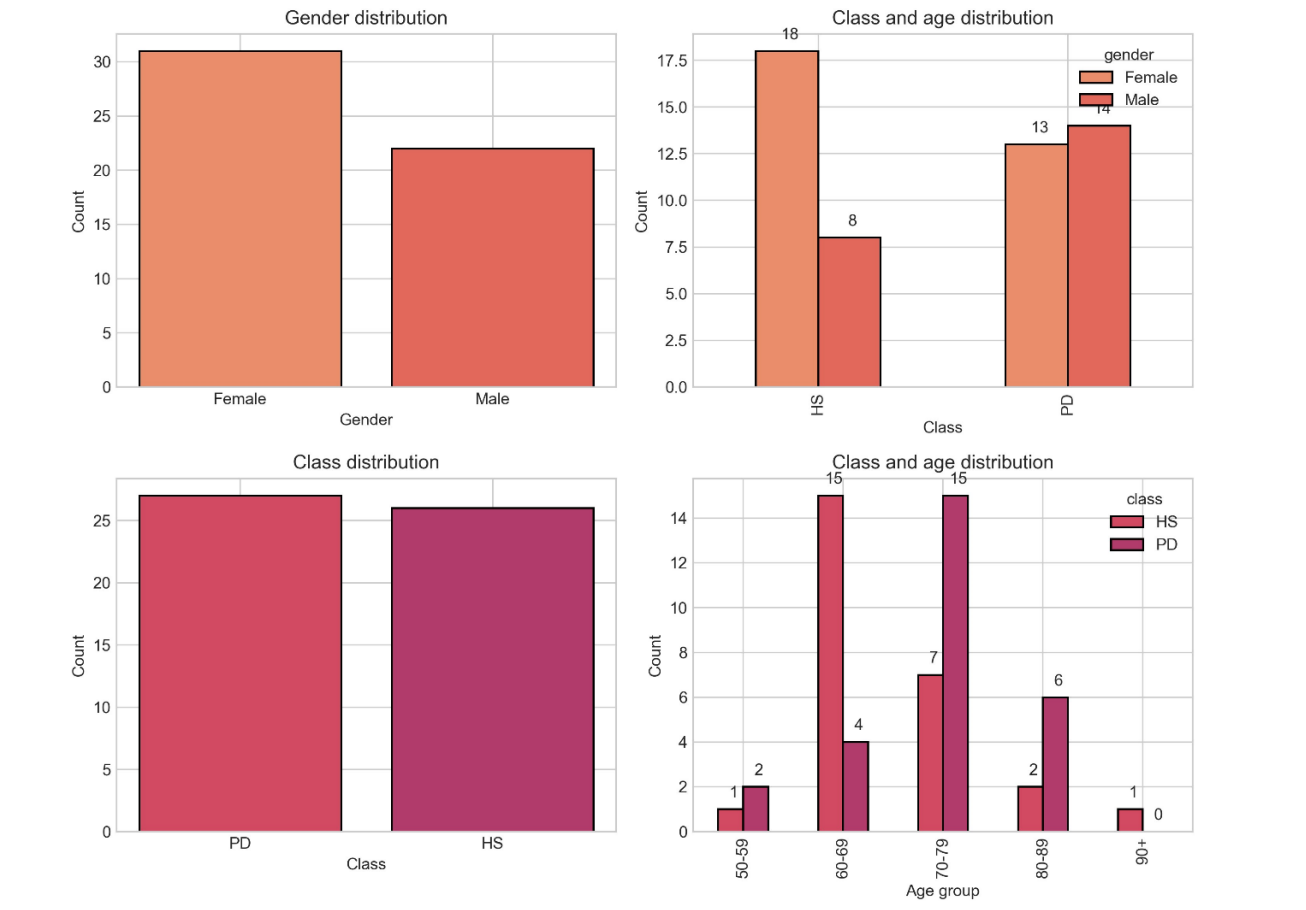
\includegraphics[width=1\textwidth]{./img/database}
%	\caption{Charakterystyka bazy danych [opracowanie własne]}
%    \label{fig:database}
%\end{figure}
%
%Starano się zachować jak najbardziej zbliżone proporcje wieku i płci pomiędzy grupą
%pacjentów a grupą porównawczą.
%Jednak ze względu na specyfikę samodzielnego zbierania danych, nie udało się osiągnąć pełnej zgodności w tym zakresie.
%Mimo to zapewniono różnorodny zbiór danych, obejmujący zarówno kobiety, jak i mężczyzn w różnych grupach wiekowych.
%Drobne różnice w liczbie próbek w poszczególnych przedziałach wiekowych nie powinny mieć istotnego wpływu na wyniki
%klasyfikacji.
%Szczegółowa charakterystyka zbioru danych została przedstawiona na Rys. \ref{fig:database}
%
%Każda osoba kwalifikująca się do badania otrzymała zadanie trzykrotnego wypowiedzenia
%samogłosek /a/, /e/, /i/, /o/ oraz /u/ w odstępach czasowych, utrzymując dźwięk przez co najmniej 2 sekundy.
%Aby zapewnić jednakowe warunki nagrywania, wyeliminowano hałasy pochodzące z
%otoczenia oraz wykorzystano pomieszczenia o podobnej akustyce.
%Wszystkie nagrania zostały zarejestrowane z częstotliwością próbkowania 44 kHz.
%Czas trwania nagrań samogłosek wynosił od 2 do 5 sekund.
%Samogłoski były nagrywane trzykrotnie dla każdej z osób.
%
%Nagrania zostały dokładnie przeanalizowane.
%Usunięto nagrania zbyt krótkie oraz te, które nie spełniały kryteriów dotyczących jakości.
%Otrzymana baza danych nadal zawierała nagrania od 27 osób chorych oraz od 26 osób zdrowych, zmieniła się jedynie liczebność nagrań dla poszczególnych
%samogłosek.
%
%Jednym z głównych celów niniejszej pracy jest przeprowadzenie analizy porównawczej
%samogłosek pod kątem ich przydatności w klasyfikacji choroby Parkinsona.
%Aby zagwarantować wiarygodność wyników, niezwykle istotne jest utrzymanie jak najbardziej zbliżonych warunków
%eksperymentalnych.
%Kluczowym aspektem tego zagadnienia jest odpowiednie dostosowanie zbiorów
%danych, ponieważ może mieć znaczący wpływ na ostateczne rezultaty analizy.
%Początkowo dysponowano zbiorem, w którym na każdą osobę zdrową przypadały trzy nagrania każdej z samogłosek, a na osobę cierpiącą na chorobę Parkinsona jedno.
%Jednak po oczyszczeniu bazy danych, liczby te uległy zmianie.
%W związku z tym, podjęto decyzję o ograniczeniu zbioru w taki sposób, aby dla każdej samogłoski uwzględniona była
%identyczna liczba nagrań pochodzących od poszczególnych osób. Ostateczny skład wybranej bazy
%danych przedstawiono w tabeli 4.1.2 oraz na wykresie 4.1.3.

%---------------------------------------------------------------------------

\section{Parametryzacja sygnału akustycznego}
\label{sec:parametryzacja-sygnalu-akustycznego}

%---------------------------------------------------------------------------

\section{Metody klasyfikacji}
\label{sec:klasyfikacja}

%---------------------------------------------------------------------------

\section{Metody ewaluacji wyników}
\label{sec:metody-ewaluacji-wyników}